% This is "sig-alternate.tex" V2.0 May 2012
% This file should be compiled with V2.5 of "sig-alternate.cls" May 2012
%
% This example file demonstrates the use of the 'sig-alternate.cls'
% V2.5 LaTeX2e document class file. It is for those submitting
% articles to ACM Conference Proceedings WHO DO NOT WISH TO
% STRICTLY ADHERE TO THE SIGS (PUBS-BOARD-ENDORSED) STYLE.
% The 'sig-alternate.cls' file will produce a similar-looking,
% albeit, 'tighter' paper resulting in, invariably, fewer pages.
%
% ----------------------------------------------------------------------------------------------------------------
% This .tex file (and associated .cls V2.5) produces:
%       1) The Permission Statement
%       2) The Conference (location) Info information
%       3) The Copyright Line with ACM data
%       4) NO page numbers
%
% as against the acm_proc_article-sp.cls file which
% DOES NOT produce 1) thru' 3) above.
%
% Using 'sig-alternate.cls' you have control, however, from within
% the source .tex file, over both the CopyrightYear
% (defaulted to 200X) and the ACM Copyright Data
% (defaulted to X-XXXXX-XX-X/XX/XX).
% e.g.
% \CopyrightYear{2007} will cause 2007 to appear in the copyright line.
% \crdata{0-12345-67-8/90/12} will cause 0-12345-67-8/90/12 to appear in the copyright line.
%
% ---------------------------------------------------------------------------------------------------------------
% This .tex source is an example which *does* use
% the .bib file (from which the .bbl file % is produced).
% REMEMBER HOWEVER: After having produced the .bbl file,
% and prior to final submission, you *NEED* to 'insert'
% your .bbl file into your source .tex file so as to provide
% ONE 'self-contained' source file.
%
% ================= IF YOU HAVE QUESTIONS =======================
% Questions regarding the SIGS styles, SIGS policies and
% procedures, Conferences etc. should be sent to
% Adrienne Griscti (griscti@acm.org)
%
% Technical questions _only_ to
% Gerald Murray (murray@hq.acm.org)
% ===============================================================
%
% For tracking purposes - this is V2.0 - May 2012

\documentclass{sig-alternate}
\usepackage{color}
\usepackage[usenames,dvipsnames]{xcolor}
\PassOptionsToPackage{hyphens}{url}\usepackage{hyperref}

\newcommand{\TODO}[1]{{\color{red} TODO: #1}}
%\newcommand{\gametitle}{{\color{RoyalPurple} Dragon Architect}}
\newcommand{\gametitle}{{\emph{Dragon Architect}}}

\toappear{Submitted for review.}

\begin{document}
%
% --- Author Metadata here ---
\conferenceinfo{Blocks and Beyond}{2015}
\pdfinfo{
  /Title (Approaches for Teaching Computational Thinking Strategies in an Educational Game: A Position Paper)
  /Author (Aaron Bauer, Eric Butler, Zoran Popovic) 
  /Subject ()
  /Keywords ()
}

\title{Approaches for Teaching Computational Thinking Strategies in an Educational Game: A Position Paper}

\numberofauthors{1} 
\author{
  \alignauthor
  Aaron Bauer, Eric Butler, Zoran Popovi\'c\\
  \affaddr{Center for Game Science}\\
  \affaddr{Computer Science \& Engineering}\\
  \affaddr{University of Washington}\\
  \affaddr{Seattle, WA 98195}
  \email{\{awb, edbutler, zoran\}@cs.washington.edu}
}

\maketitle
\begin{abstract}
Computer science is expanding into K12 education and numerous educational games and systems have been created to teach programming skills, including many block-based programming environments. Teaching computational thinking has received particular attention, and more research is needed on using educational games to directly teach computational thinking skills. We propose to investigate this using \emph{Dragon Architect}, an educational block-based programming game we are developing. Specifically, we wish to study ways of directly teaching computational thinking strategies such as divide and conquer in an educational game, as well as ways to evaluate our approaches. 
\end{abstract}

\section{Introduction}

Teaching \emph{computational thinking} has been a focus of recent efforts to broaden the reach of computer science education, including those using block-based programming environments. 
In their review of recent literature on teaching computational thinking, Lye and Koh~\cite{lye2014review} use Brennan and Resnick's definition of computational thinking as consisting of \emph{concepts}, \emph{practices}, and \emph{perspectives}~\cite{brennan2012new}. 
Concepts are basic programming ideas (such as variables, conditionals, and loops), practices are the problem-solving strategies used while programming (such as ``being incremental and iterative'' or ``using abstraction and modularization''), and perspectives are the relationships with the wider technological world. 
Lye and Koh conclude that more research is needed on teaching computational thinking \emph{practices} in particular. 
How to \emph{directly} teach such skills in is an open problem, including in the context of a block-based programming environment. 

In this paper we propose investigating directly teaching computational practices in an educational block-based programming game called \emph{Dragon Architect}. 
We briefly discuss existing work on teaching computational thinking and the direct teaching of problem-solving strategies. 
We describe ways this might be attempted in \emph{Dragon Architect}, as well as ways we might evaluate such work. 

\section{Game Description}

Before we discuss teaching computational thinking, we describe basic information about \emph{Dragon Architect}\footnote{Play the game at \url{http://centerforgamescience.org/portfolio/dragon-architect}.\\\\Source code available at \url{http://gigantor.cs.washington.edu/dragon-architect-source.zip}.} to provide context for the discussion.
In \emph{Dragon Architect}, players write code to control a dragon that builds 3D structures in a block world.
Our game, which has been in development since spring 2014, is played in a web browser.
Similar to other programming environments, the user interface is separated into two parts: an area where the player can assemble their code and a visualization of the 3D environment their code affects (see Figure~\ref{fig:overall}). 
The game uses the block-based programming library Blockly~\cite{blockly} for inputing code.

The player can write programs to move the dragon in three dimensions and have the dragon place and remove cubes of various colors. 
In addition to blocks that control the dragon directly, players can also use definite loops and procedures (see Figure~\ref{fig:toolbox}).
As players progress through the game, they alternate between short sequences of puzzles with a specific goal and constrained set of available code blocks and an open-ended sandbox.
The game begins with puzzles that introduce the idea of assembling and running code, as well as the code blocks for moving the dragon and placing cubes.
After that, the player can creatively experiment and build in the sandbox and complete other puzzle sequences to make more code blocks available, switching between sandbox and puzzles at any time. 
In this way, the language the player uses to write instructions for the dragon gradually expands as the player advances.

The popularity and uniquely broad appeal of \emph{Minecraft}~\cite{minecraft} motivated our use of a 3D grid world in which the player's programs could place cubes.
This choice also makes it natural to extend our game in the future with exploration, more complex interaction with the environment, or players working together in a shared world.
Our playtests with \emph{Dragon Architect} have shown the premise of programming a dragon in a \emph{Minecraft}-like world appeals to younger players of all genders.
Common sandbox activities have included making the dragon travel very long distances, building big and impressive towers, and spelling one's name out of cubes.

\begin{figure*}[t!]
  \centering
  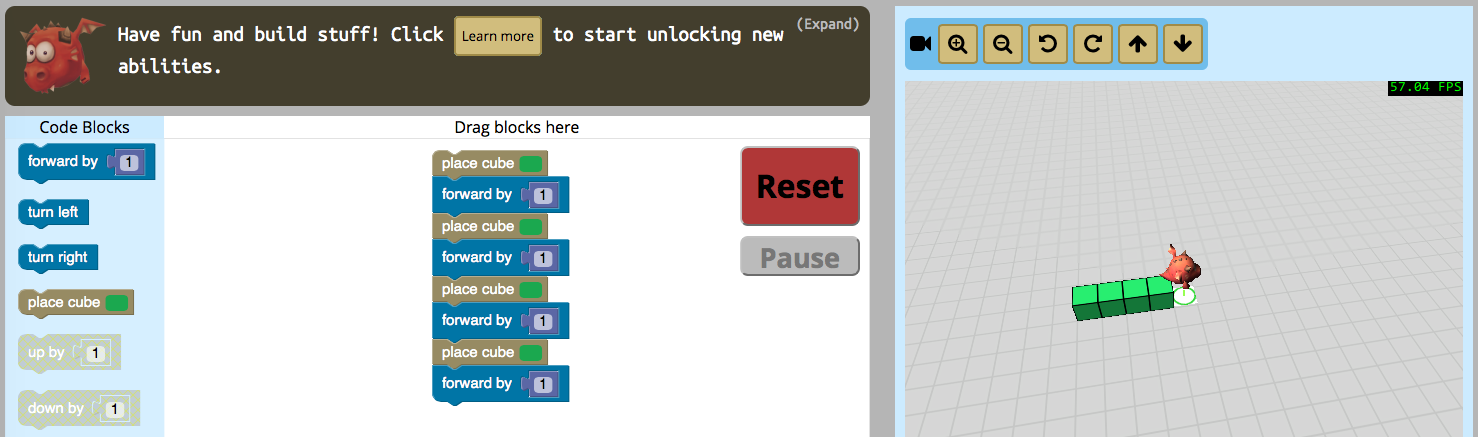
\includegraphics[width=\textwidth]{images/overall-example-cropped}
  \caption{The player assembles code to control the dragon on the left side, and the dragon and world it inhabits are visualized on the right side. Only a few different code blocks are available to the player initially, and more are unlocked through completing guided puzzles.}
  \label{fig:overall}
\end{figure*}

\begin{figure}[htb]
  \centering
  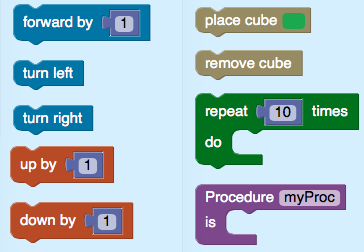
\includegraphics[width=\columnwidth]{images/toolbox-wide}
  \caption{The programming elements available in \gametitle{}, which include moving the dragon, placing blocks, definite loops, and procedure definitions.}
  \label{fig:toolbox}
\end{figure}

\section{Teaching Computational Thinking Strategies}

% what is it
Many have studied how to increase the presence and effectiveness of computational thinking in computer science education and education in general (e.g., Barr and Stephenson~\cite{barr2011bringing}, Grover and Pea~\cite{grover2013computational}). 
Furthermore, educational games and other systems often have teaching computational thinking as an explicit goal (e.g., Weintrop and Wilensky~\cite{weintrop2013robobuilder},  Kazimoglue et al.~\cite{kazimoglu2012serious}) or have a computational thinking framework built around them (e.g., Gouws et al.~\cite{gouws2013lightbot}, Computational Thinking with Scratch~\cite{scratchedCT}).
A recent review of the literature on teaching computational thinking found that additional empirical research is needed~\cite{lye2014review}, particularly in the case of computational thinking practices.
In addition, we believe using educational games to teach computational thinking skills deserves to be the focus of more empirical work. 

% how can we teach it directly?
Specifically, we propose to investigate directly teaching computational thinking strategies in \emph{Dragon Architect}. 
Simply playing in a computational environment where these strategies are necessary is unlikely to teach students such complex skills~\cite{mayer2004should}.
Instead, we must address how to directly teach computational thinking skills by investigating which guidance is effective and how it is best deployed in an educational game.
One such skill is the identification and application of problem-solving strategies, which is a core component of computational thinking.
A great deal of recent education research suggests that ``curricula can model such strategies for students'' and that appropriate guidance can ``enable students to learn to use these strategies independently''~\cite{report2010computational}.
Mayer and Wittrock call attention to the substantial evidence in the education literature for teaching what they call \emph{domain-specific thinking skills} and \emph{metacognitive skills}~\cite{mayer1996handbook}.
The former would include the ability to use a strategy like divide and conquer, and the latter would include knowing when and where to employ that strategy.
In both cases, Mayer and Wittrock describe studies (for non-computer science domains) that have shown teaching these skills directly can improve learning and performance. 
It is an open question whether this can be applied to teaching computational thinking in a game.

% teaching stategies like divide and conquer
One computational thinking strategy we intend to focus on in \emph{Dragon Architect} is \emph{divide and conquer}.
One potential approach is to lead the player though a top-down deconstruction of building a castle in order to model iteratively subdividing a large problem into more manageable subproblems.
The player is presented with a single code block that builds an entire castle, but discovers the construction has a number of flaws. 
The next several puzzles each decompose some part of the flawed program in order to give the player a chance to repair it. 
For example, to enable the player to give the castle the correct number of walls and towers, the castle code block is split into a tower block and a wall block that the player uses to write a corrected castle procedure, as shown Figure~\ref{fig:decomp}. 

\begin{figure*}[th!]
  \centering
  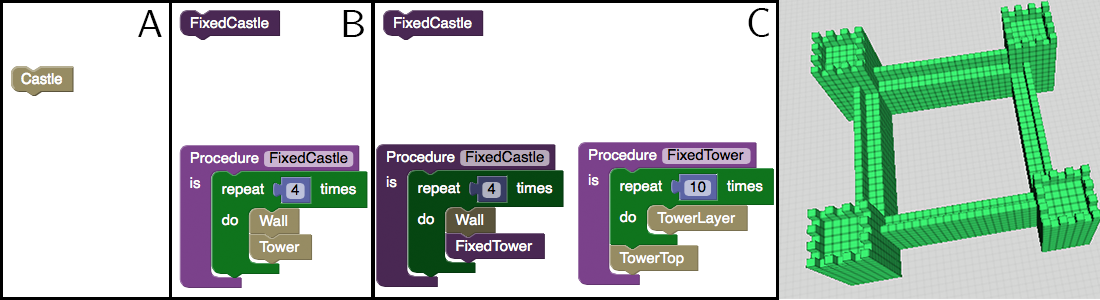
\includegraphics[width=\textwidth]{images/decomp-code}
  \caption{The code required by a progression of levels demonstrating the strategy of divide and conquer. In A, the player uses a single code block to build an entire castle. Then, in B, the player is given an empty \texttt{FixedCastle} procedure, which they must fill with the appropriate number of wall and tower blocks. Finally, in C, the player is given a completed \texttt{FixedCastle} procedure and must fill in the \texttt{FixedTower} procedure as shown. The final completed castle is shown on the right.}
  \label{fig:decomp}
\end{figure*}

A companion approach is a gradual bottom-up progression modeling the combining of the blocks currently available to the player into more sophisticated constructs. 
For example, the player is tasked with writing a program to place a line of cubes. 
When this is completed, the player is awarded a new kind of block that by itself places a line of cubes (i.e., a block encapsulating the player's previous program). 
Subsequent puzzles ask the player to use the line block to construct other, more complicated structures, each time granting the player a single, encapsulating block.  

Evaluating learning outcomes and other effects of these or similar approaches is a tremendous challenge. 
Computational Thinking with Scratch proposes three kinds of assessment: (1) artifact-based interviews, (2) design scenarios, and (3) learner documentation~\cite{scratchedCT}. 
We believe these to be promising, and worthy of further study. 
In addition to design scenarios, we propose that more general kinds of in-game assessments could be useful. 
Like Scratch, \emph{Dragon Architect} provides users a place for unstructured creative exploration. 
The effectiveness of an attempt to directly teach computational thinking strategies could be assessed by comparing the programs written by those who completed the relevant puzzles to those who did not (after controlling for time played, and differences in programs prior to completing the puzzles).
A variety of other in-game metrics could contribute to an assessment including a player's solutions to specific challenges, time taken to complete puzzles, etc. 

On-paper assessments (given as pre-test and post-test) could also serve as an evaluation.
Computational thinking skills might be assessed through language-independent assessments of computer science knowledge~\cite{tew2011fcs1} or general problem-solving assessments such as those developed by the Program for International Student Assessment~\cite{pisa}. 
Finally, Grover and Pea suggest ``academic talk'' (i.e., student development and use of computational language) could be leveraged as an additional assessment of computational thinking~\cite{grover2013computational}. 

% Comment out in submission version
%\section{Acknowledgments}
%\TODO{copy from CHI papers?}

\bibliographystyle{abbrv}
\bibliography{dragon-architect-vlhcc-2015} 
\end{document}
